\section{Path-consistency}
\label{sec:method}
Path-consistency reduces repeated reasoning by reusing a continuous prefix across sampling windows and testing its extensions with subsequent samples. Its three components are answer agreement, prefix selection, and trial and recovery, as illustrated in Figure~\ref{fig:loop} and described below. Figure~\ref{fig:overview} shows the overall workflow. The default main setting uses a trajectory budget $B=32$, window size $m=4$, and prefix levels $\mathcal R=\{0,0.2,0.4,0.6,0.8\}$. A prefix level $r\in\mathcal R$ specifies the nominal fraction of the source trajectory's reasoning tokens retained as the shared prefix, excluding the final answer. For example, $r=0.2$ retains approximately the first 20\% of that reasoning, while $r=0$ means no prefix reuse. All trajectories within a window use the same prefix. Path-consistency updates its prefix and agreement statistics only after all trajectories in that window have finished. Self-consistency and path-consistency use the same maximum budget and final majority-vote rule.

\begin{figure}[t]
\centering
% Author-redrawn vector panels supplied in figs/.
% Equal image heights preserve aspect ratios and align all caption baselines.
\begingroup
\edef\PCMethodPanelHeight{\the\dimexpr0.403\linewidth\relax}
\begin{minipage}[t]{0.31\linewidth}
\vspace{0pt}\centering
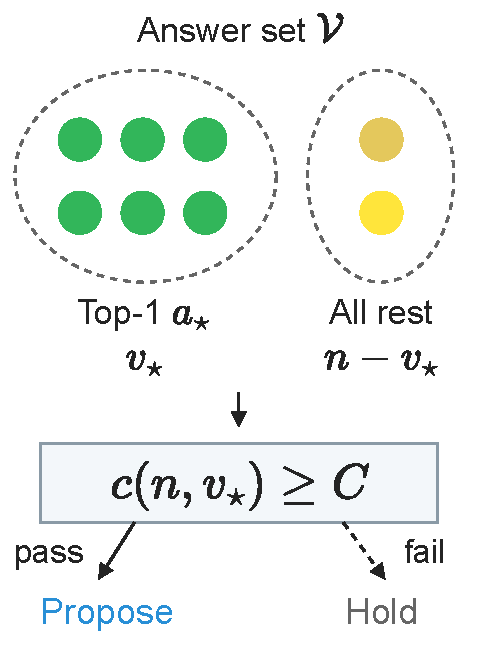
\includegraphics[height=\PCMethodPanelHeight]{figs/method_1.pdf}
\par\smallskip
{\small\textbf{(a) Answer agreement}}
\end{minipage}\hfill
\begin{minipage}[t]{0.326\linewidth}
\vspace{0pt}\centering
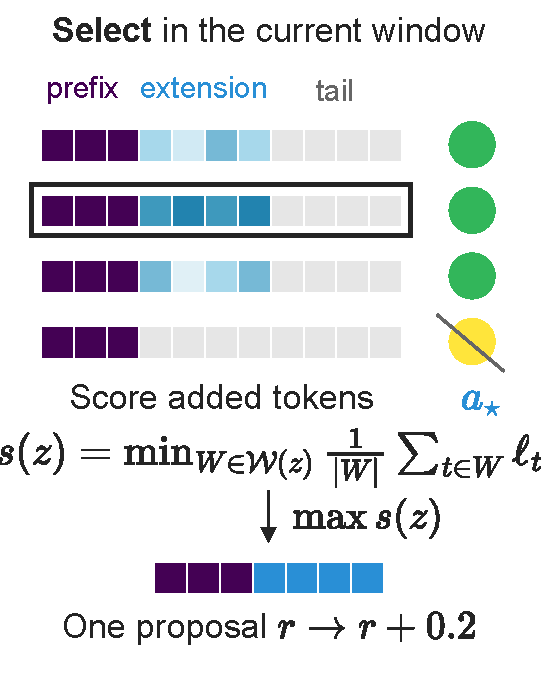
\includegraphics[height=\PCMethodPanelHeight]{figs/method_2.pdf}
\par\smallskip
{\small\textbf{(b) Prefix selection}}
\end{minipage}\hfill
\begin{minipage}[t]{0.332\linewidth}
\vspace{0pt}\centering
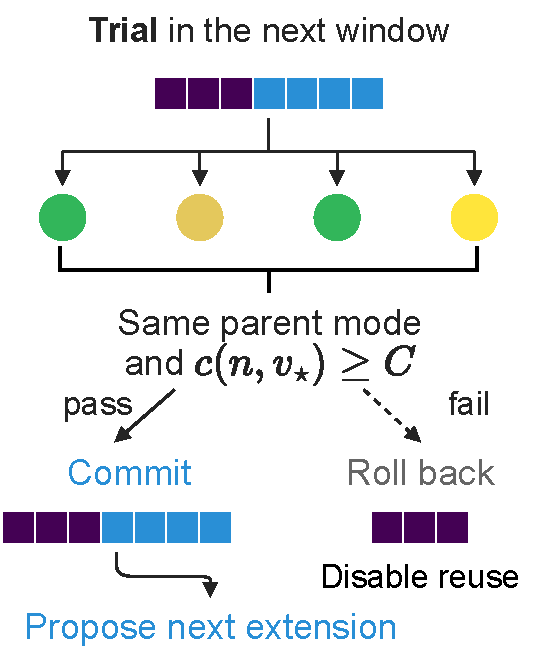
\includegraphics[height=\PCMethodPanelHeight]{figs/method_3.pdf}
\par\smallskip
{\small\textbf{(c) Trial and recovery}}
\end{minipage}
\endgroup

\caption{The three components of PC. (a) Answer agreement determines whether to propose a prefix extension. (b) Local confidence selection chooses an extension from eligible trajectories. (c) Trial and recovery validate the proposal, enabling further extension on success or returning to an earlier prefix on failure. Purple denotes inherited prefixes and blue denotes new extensions. Circles represent answers, with colors indicating answer categories.}
\label{fig:loop}
\end{figure}

\subsection{Answer agreement gate}
Let $\mathcal V$ contain the valid answers admitted by previous successful windows, let $n=|\mathcal V|$, and let $v_\star$ be the count of its modal answer $a_\star$. We use the top-1-versus-all-rest score
\begin{equation}
 c(n,v_\star)=1-I_{1/2}(v_\star+1,n-v_\star+1),
 \label{eq:beta}
\end{equation}
where $I_x$ is the regularized incomplete beta function. For a \emph{fixed} answer category with independent Bernoulli observations and a uniform prior, this is the posterior probability that its mass exceeds $1/2$. In path-consistency the category is selected from the data, successive windows use different prefixes, and unsuccessful windows are excluded from $\mathcal V$. Thus Equation~\ref{eq:beta} is an operational agreement score, not a calibrated posterior over correctness or an anytime error bound.

A nonempty answer set with $c\geq C$ permits a proposal. We fix $C=0.8$ in the main experiments as the default operating point, without selecting it on a development or test set. Threshold sweeps are sensitivity analyses only. At $C=1$ no finite-sample Beta score reaches the threshold in exact arithmetic, recovering self-consistency. A setting of $C=0$ removes the confidence barrier but still requires a valid modal answer and a feasible prefix.

\subsection{Selecting a single continuous prefix}
Once answer agreement permits an extension, path-consistency selects a source trajectory from the just-completed, accepted window. Eligible trajectories must support the modal answer $a_\star$. For a current prefix level $r<0.8$, each trajectory proposes a candidate prefix $z$ ending at $\lfloor(r+0.2)L\rfloor$, where $L$ counts all reasoning tokens in that trajectory, including the inherited prefix but excluding the final answer. Thus each proposal targets the next 20\% level while preserving the existing prefix. The endpoint may be moved backward by up to 32 tokens to avoid explicit answer markers and unbalanced braces or code fences, with punctuation boundaries preferred. Only candidates that extend the current prefix are retained.

We use local confidence selection to rank these candidates using only their newly added tokens. Let $\ell_t$ be the log probability assigned to token $t$ when it was sampled, and let $\mathcal W(z)$ contain the sliding token windows over the added segment of candidate $z$. We define
\begin{equation}
 s(z)=\min_{W\in\mathcal W(z)}\frac{1}{|W|}\sum_{t\in W}\ell_t,
 \label{eq:blc}
\end{equation}
where $W$ is a token window and $|W|$ is its number of scored tokens. The score is the lowest mean log probability across these windows, so choosing the largest $s(z)$ favors candidates whose least confident segment has the highest score. Scoring excludes the inherited prefix, which is shared by all candidates. We use windows of 128 tokens with stride 64 and include the final window; segments shorter than 128 tokens are scored as a whole.

Ties are resolved by fewer generated source tokens and then branch ID. Missing or nonfinite log probabilities are omitted. A candidate with no usable scores receives $-\infty$, and if all candidates receive this value, the same tie-breaking rule selects the source.

\subsection{Trial, commitment, and rollback}
As illustrated in Figure~\ref{fig:loop}(c), a proposed prefix is used for the next sampling window as a trial. After that window finishes, we compute the agreement score in Equation~\ref{eq:beta} using $\mathcal V$ together with the trial's valid answers. The trial succeeds if the modal answer remains the same as when the prefix was proposed and the score is at least $C$. We then commit the prefix, add the trial's valid answers to $\mathcal V$, and reset the consecutive-failure counter.

The same agreement score also gates the next prefix extension. Since a successful trial has already met the threshold, no additional agreement calculation is needed after commitment. If sampling budget remains and the prefix level is below 0.8, the accepted window supplies candidate extensions at the next level using the selection procedure above. A feasible selected extension becomes the next trial; otherwise, sampling continues with the committed prefix. Thus one window can both validate the preceding proposal and supply the next extension.

If a trial fails, we discard its proposed prefix and return to the last committed prefix. A failed monitoring window at an already committed prefix rolls back one level. Two consecutive failures clear the prefix stack and disable further prefix reuse for that question. Failed-window answers are excluded from subsequent agreement calculations and source selection, but all valid answers still contribute to the final vote and the full generation cost is counted. Earlier admitted answers remain in $\mathcal V$ after rollback.

At root, valid answers enter $\mathcal V$ even if confidence is too low to propose a prefix. The algorithm stays at the current level when there is no feasible extension, and cannot extend past the nominal 80\% level. Because each new source can have a different length, a level is a fraction of that source, not a fixed absolute number of tokens. Appendix~\ref{app:algorithm} gives the state transitions used in the runs.
